\section{Results and Discussion}\label{sec:results}
For each unique configuration yielded by varying the parameters, BER versus $\text{SNR}^{\text{tx}}_{\text{avg}}$ is empirically determined using monte-carlo simulations. Based on the simulation setup, the path-loss from the transmitting elements to the receiving elements is about 145 dB. To plot the change in system performance when each parameter is varied, the minimum $\text{SNR}^{\text{tx}}_{\text{avg}}$ needed to achieve target BER $\leq 10^{-3}$ is selected. Since ACO-OFDM is more power efficient compared to DCO-OFDM, for all the cases discussed below, ACO-OFDM needs lower transmit signal power to achieve the target BER as compared to DCO-OFDM.

%\begin{figure}[!b]
	%\centering
		%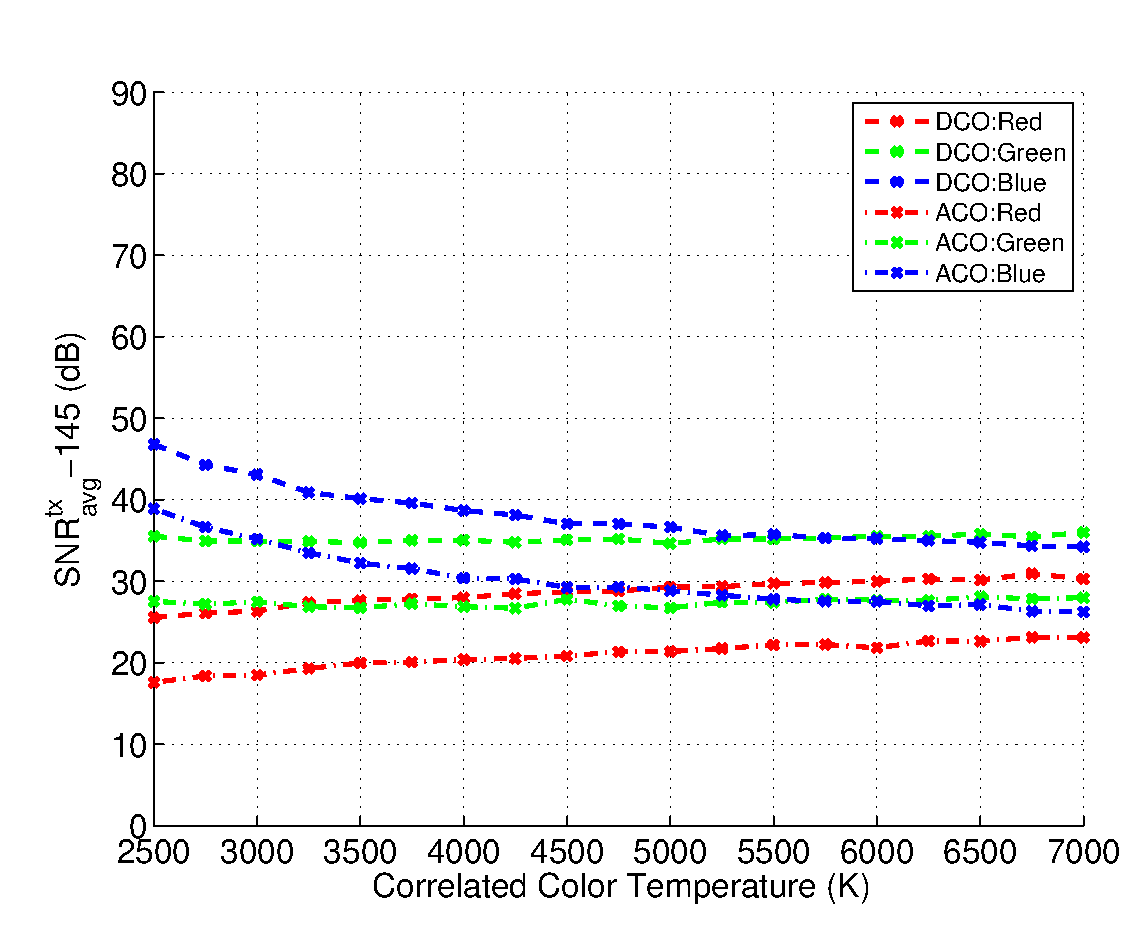
\includegraphics[trim={0.15in 0.05in 0.05in 0.35in}, clip=true, width=2.9in]{img/SNRvsCCT.eps}
	%\caption{$\text{SNR}^{\text{tx}}_{\text{avg}}$ vs correlated color temperature to achieve BER $\leq 10^{-3}$\newline Transmitter: $\sigma_r = \sigma_g = \sigma_b = 5$ nm; Filter: $\Gamma_r = \Gamma_g = \Gamma_b = 40$ nm}
	%\label{fig:SNRvsCCT}
%\end{figure}


The change in performance of the red, green and blue links as the CCT is varied from 2500 K to 7000 K is shown in \figurename{\ref{fig:SNRvsCCT}}. At 2500K, the SPD has a greater contribution from red, then green and then blue. Thus the red link achieves target BER at lower transmitted signal power. As the CCT increases, relative signal power from the red link decreases, that of the green remains similar, and that of the blue increases. Thus the amount of aggregate transmit flux needed to achieve target BER from the red link starts increasing, that of the green remains relatively unchanged, while that of the blue decreases with increase in CCT. For the specified multi-wavelength system, CCT = 6250 K provides the most power efficient operating point as illustrated in \figurename{\ref{subfig:SNRvsCCThigh}}. Increasing the transmitting elements' SPD or the filter FWHM introduces increasingly more inter-channel interference (ICI). This causes the most power efficient operating point to shift towards CCT = 3500 K but with greater power requirements as seen in \figurename{\ref{subfig:SNRvsCCTlow}}.

\begin{figure}[!b]
	\centering
		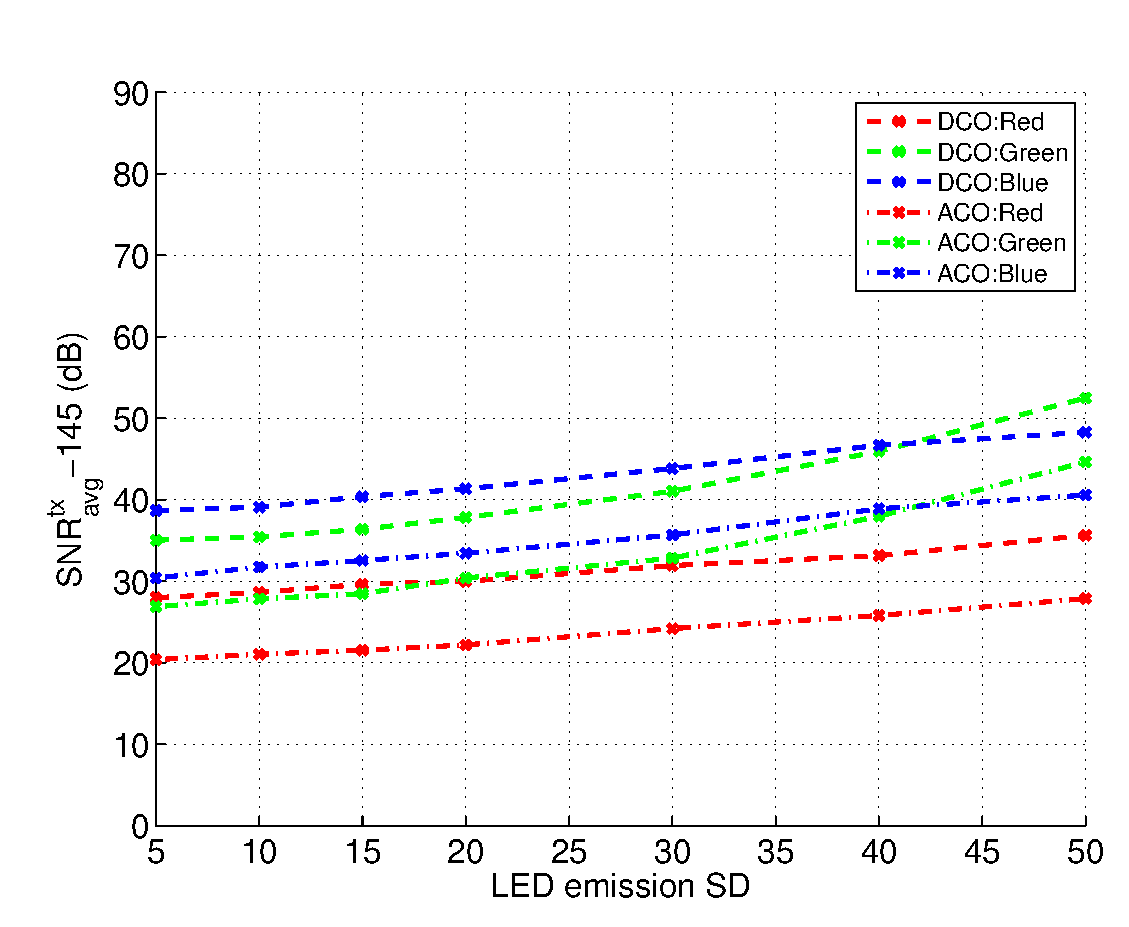
\includegraphics[trim={0.15in 0.05in 0.05in 0.35in}, clip=true, width=2.9in]{img/SNRvsLEDSD.eps}
	\caption{$\text{SNR}^{\text{tx}}_{\text{avg}}$ vs transmitting element spectral power distribution spread to achieve BER $\leq 10^{-3}$\newline Filter: $\Gamma_r = \Gamma_g = \Gamma_b = 40$ nm; CCT = 6250 K}
	\label{fig:SNRvsLEDSD}
\end{figure}

The change in performance of the red, green and blue links as the transmitting element SPD spread is varied from 5 nm to 50 nm is shown in \figurename{\ref{fig:SNRvsLEDSD}}. As the SPD spread is increased, the performance of all three links degrade. This can be attributed to two factors. Initially, as the signal power is distributed across a larger wavelength range, with the filter transmittance function remaining the same, increasingly more signal gets rejected by the filter. Thus the receiver collects a smaller fraction of the signal power, degrading the performance. Secondly, as the individual SPDs spread enough, they start overlapping and causing ICI. The effect of ICI is more pronounced on the green link because it gets interference from both, red and blue. Thus transmitter consisting of transmitting elements with narrower emission spectra are more power efficient efficient than those with wider emission spectra. Experiments in reference \cite{neu11a} qualitatively measure color perception for illumination with narrow-band sources and find lasers could be used for general lighting. However, it is also commonly believed that sources with spiky emission spectra do not produce good quality of illumination because objects with reflectance spectra lying outside the spikes in the illumination spectra will be perceived to be poorly lit. The choice of the transmitting elements' SPD spread would be a tradeoff between the communication and illumination performance. For the specified multi-wavelength system, SPD spread = 5 nm provides the most power efficient operating point.

The change in performance of the red, green and blue links as the receiving element filter FWHM is varied from 1 nm to 250 nm is shown in \figurename{\ref{fig:SNRvsFLTWID}}. As the filter FWHM increases, initially the system performance improves significantly. At these lower FWHM ranges, the filters transmit a smaller fraction of the signal to the sensors and thus performance is limited by the amount of signal power collected for each link. At higher FWHM ranges, along with additional signal, the filters permit increasingly more ambient light and interference from neighboring links, thus degrading the performance. For the specified multi-wavelength system, filter FWHM = 40 nm provides the most power efficient operating point.

\begin{figure}[!t]
	\centering
		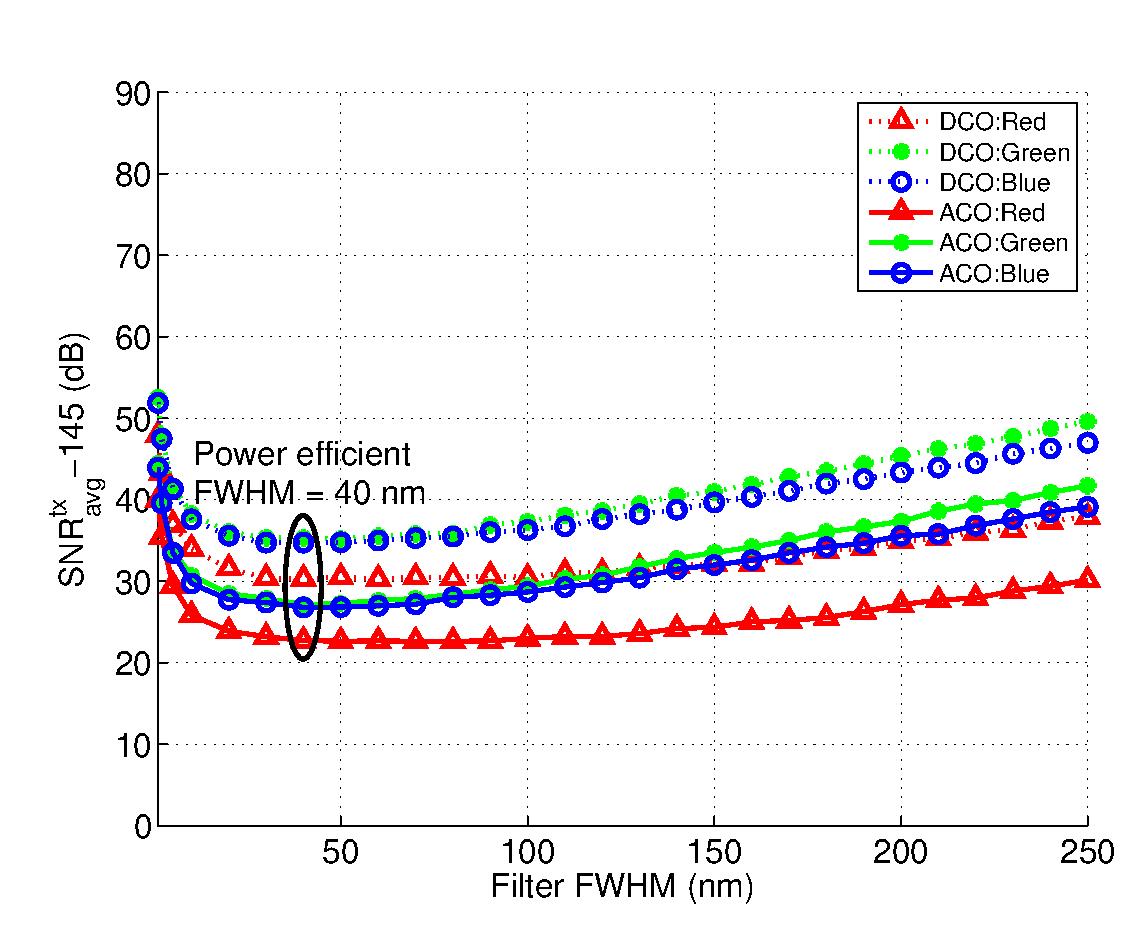
\includegraphics[trim={0.15in 0.05in 0.05in 0.35in}, clip=true, width=2.9in]{img/SNRvsFLTWID.eps}
	\caption{$\text{SNR}^{\text{tx}}_{\text{avg}}$ vs filter full width at half maximum to achieve BER $\leq 10^{-3}$\newline Transmitter: $\sigma_r = \sigma_g = \sigma_b = 5$ nm; CCT = 6250 K}
	\label{fig:SNRvsFLTWID}
\end{figure}










